
\documentclass[]{tukediphc}
\pdfoutput=1
%% -----------------------------------------------------------------
%% tento subor ma kodovanie utf-8
%%
%% na kompilaciu pouzivajte format pdfcslatex 
%%
%% vytvorene distribuciou texlive 2009-7
%% -----------------------------------------------------------------
\usepackage[utf8]{inputenc}
%\usepackage[T1]{fontenc}
\usepackage{lmodern,textcase}
\usepackage{slovak}\renewcommand{\figurename}{Obr\'azok}
\def\refname{Zoznam pou\v{z}itej literat\'ury}
\usepackage{latexsym}
\usepackage{dcolumn} % zarovnanie cisiel v tabulke podla des. ciarky
\usepackage{hhline}
\usepackage{amsmath}
\usepackage{nicefrac} % pekne zlomky
\usepackage{upgreek} % napr. $\upmu\mathrm{m}$ pre mikrometer ...
\usepackage[final]{showkeys}%color%notref%notcite%final
\usepackage[slovak,noprefix]{nomencl}
\makeglossary % prikaz na vytvorenie suboru .glo
%\usepackage{parskip}% 'zhusti' polozky obsahu
\usepackage{indentfirst}
%%
%\usepackage[dvips]{graphicx}
%\DeclareGraphicsExtensions{.eps}
\usepackage[pdftex]{graphicx}
\DeclareGraphicsExtensions{.pdf,.png,.jpg,.mps}
\graphicspath{{figures/}} % priecinok na obrazky
%%
%% Cislovane citovanie
%\usepackage[numbers]{natbib}
%%
%% Citovanie podľa mena autora a roku
\usepackage{natbib} \citestyle{chicago}
% -----------------------------------------------------------------
%% tlač !!!
\usepackage[pdftex,unicode=true,bookmarksnumbered=true,
bookmarksopen=true,pdfmenubar=true,pdfview=Fit,linktocpage=true,
pageanchor=true,bookmarkstype=toc,pdfpagemode=UseOutlines,
pdfstartpage=1]{hyperref}
\hypersetup{%
baseurl={http://www.tuke.sk/sevcovic},
pdfcreator={pdfcsLaTeX},
pdfkeywords={Optimaliz\'acia, diplomov\'a pr\'aca, p\'isanie},
pdftitle={Optimalizácia písania diplomových prác},
pdfauthor={J\'an Zelen\'y},
pdfsubject={Bakalárska práca}
} 
%% nehodiace zakomentujte !
%\dippraca{Diplomová práca}
\bakpraca{Bakalárska práca}
%%
\nazov{Inventárny systém pre platformu Android}
%% ked praca nema 'podnazov' zakomentujte nasledujuci riadok
%% alebo polozku nechajte prazdnu
%\podnazov{}
\autor{Vlastimil Brečka}
\veduciprace{Ing.~Peter~Feciľak, PhD.}
\konzultanta{Ing.~Peter~Feciľak, PhD.}
%\konzultantb{}
\univerzita{Technická univerzita v~Košiciach}
\fakulta{Fakulta elektrotechniky a informatiky}
\skratkafakulty{FEI}
\katedra{Katedra počítačov a informatiky}
\skratkakatedry{KPI}
\odbor{9.2.1 Informatika}
\specializacia{Informatika}
\abstrakt{Cieľom bakalárskej práce bol návrh a implementácia aplikácie inventárneho systému pre platformu Android. Aplikácia je schopná prevziať aktuálny inventárny zoznam zo servera, ktorý je možno členiť do osobitých miestností. Kontrola inventáru prebieha načítaním QR kódu umiestneného na predmete pomocou vstavanej kamery mobilného telefónu a jeho následným spracovaním aplikáciou. Aplikácia má následne možnosť exportovať výsledky invetúry v podobe správy vo formáte HTML na server alebo lokálne na SD-kartu a rozoslať e-mailové notifikácie.}
\klucoveslova{Inventárny systém, inventúra, Android, QR kód}
\abstrakte{The goal of bachelor‘s work was to design and implement inventory system application for Android platform. Application is able to download current inventory list from server and divide it into separate rooms. The actual inventory lookup is performed by scanning the QR code, placed on the item, via mobile phone‘s embedded camera and processing its content by the application. Upon completion, the application is able to export results as a HTML report to server or locally to phone's SD-card and send out e-mail notifications.}
\keywords{Inventory system, inventory lookup, Android, QR code}
\datumodovzdania{25. 5. 2012}
\mesto{Košice}

\begin{document}
\renewcommand\theHfigure{\theHsection.\arabic{figure}}
\renewcommand\theHtable{\theHsection.\arabic{table}}
\bibliographystyle{dcu}

\prvastrana

\titulnastrana

\abstraktsk % abstrakt v SK 

\abstrakteng % abstrakt v ENG

\kabstrakt % koniec abstraktov, nova strana

% Na tomto mieste bude vložené zadanie diplomovej práce
\zadanieprace

\cestnevyhlasenie
% Niektorí autori metodických príručiek o~záverečných prácach sa
% nazdávajú, že takéto vyhlásenie je zbytočné, nakoľko povinnosť
% vypracovať záverečnú prácu samostatne, vyplýva študentovi zo zákona a
% na autora práce sa vzťahuje autorský zákon.

\podakovanie
Chcel by som vyjadriť poďakovanie vedúcemu práce Ing. Petrovi Feciľakovi, PhD. za pripomienky pri vypracovaní práce a Branislavovi Dlugošovi za zapožičanie zariadenia mobilného telefónu.
\kpodakovania

\predhovor

Dlhotrvajúci trend vzrastajúcej popularity smartfónov v dnešnej dobe dáva možnosť a priestor softvérovým vývojárom ako ovplyvniť ďalšiu sféru ľudského života.

Hlavný dôvod, ktorý ma viedol k výberu témy je aktuálnosť modernej problematiky a predchádzajúci záujem o vytváranie aplikácií pre platformu Android. Značné rozšírenie platformy Android zväčšuje možný dosah používateľov pre danú aplikáciu. Znalosť platformy dáva možnosť vývojárom osloviť týchto potencionálnych zákazníkov poskytnutými riešeniami, rozšíriť svoje portfólio prác a zlepšiť takto svoju pozíciu na trhu práce. Bakalársku prácu som preto považoval za vhodnú príležitosť ako si plne osvojiť túto inak veľmi zaujímavú tému aj z praktických dôvodov.

Cieľom tejto práce je návrh a implementácia aplikácie inventárneho systému pre mobilnú platformu Android, ktorá zjednoduší a zefektívni procesy potrebné pri inventúre na katedre. Použité moderné postupy vykonávania inventúry sprehľadňujú a urýchľujú inak zdĺhavý úkon inventúry. Poskytnuté riešenia umožňujú taktiež jednoduchú a nenáročnú archiváciu.

V práci sa taktiež venujem stavbe operačného systému Android a teórií vývoja a základnej štruktúre vytváraných aplikácií. 

\kpredhovoru

\thispagestyle{empty}
\tableofcontents
\newpage

\thispagestyle{empty}
%\addcontentsline{toc}{section}{\numberline{}Zoznam obrázkov}
\listoffigures
\newpage

\thispagestyle{empty}
%\addcontentsline{toc}{section}{\numberline{}Zoznam tabuliek}
\listoftables
\newpage

\thispagestyle{empty}
%\addcontentsline{toc}{section}{\numberline{}Zoznam symbolov a
%skratiek}
\printglossary % vlozenie zoznamu skratiek a symbolov
\newpage

%\addcontentsline{toc}{section}{\numberline{}Slovník termínov}
\slovnikterminov

\begin{description}

	\item[Operačný systém] je softvér, ktorý spravuje zdroje počítača
a poskytuje programátorom rozhranie pre prístup k týmto zdrojom. Operačný
systém tiež spracúva dáta a a vstupy od používateľa a odpovedá alokovaním
a spravovaním úloh a interných zdrojov počítača ako služby pre používateľa.

	\item[Používateľské rozhrania] sú programy a zariadenia, ktoré sú k dispozícií používateľovi systému na spracovanie dát.

	\item[Java] je objektovo orientovaný programovací jazyk. Je vyvíjaný spoločnosťou Oracle. Jeho syntax vychádza z jazykov C a C++. Zdrojové programy sa nekompilujú do strojového kódu, ale do medzistupňa, tzv. bajt kódu, ktorý nie je závislý na konkrétnej platforme.

\item[Softvérový vývojový balíček] je súhrn nástrojov pre vývoj softvéru, ktorý umožňuje vytváranie aplikácií pre určitú platformu, framework, operačný systém.

	\item[Debugovanie] je metodologický proces hľadania a redukovania počtu chýb a defektov v počítačovom programe s cieľom zabezpečenia korektného chovania aplikácie.

	\item[Virtuálny stroj] je softvér, ktorý vytvára virtualizované prostredie medzi platformou počítača a operačným systémom, v ktorom koncový používateľ môže používať softvér na abstraktnom stroji.
Framework je softvérová štruktúra, ktorá slúži na podporu programovania a vývoj iných softvérových projektov. Môže obsahovať podporné programy, knižnice API alebo podporu pre návrhové vzory.

\end{description}

\kslovnikterminov
%
\setcounter{page}{1}
\setcounter{equation}{0}
\setcounter{figure}{0}
\setcounter{table}{0}

\section*{\'Uvod}
\addcontentsline{toc}{section}{\numberline{}\'Uvod}
	Rozmach smartfónov a tabletov v poslednej dobe zmenil tieto zariadenia na neoddeliteľnú súčasť ľudského života a predmety dennej potreby. Mobilný telefón je jediné zariadenie, ktoré skutočne ľudia nosia neustále so sebou, čo má veľký dopad na potenciál a možnosti možných programov, pre nich určené. Tento poznatok, spolu s fenoménom internetu a dotykovým displejom, ktorý predstavuje skutočne prirodzenú formu interakcie so zariadením, z nich tvorí ideálny prostriedok komunikácie rôzneho druhu.

	Neustály vývoj v hardvérovej oblasti podmieňuje vývoj v oblasti softvérovej do takej miery, že poskytnutý výkon umožňuje využívať takmer všetky z moderných technológií, známych zo sféry stolných počítačov. To spôsobuje možnosť jednoduchého prechodu programátorov na mobilné platformy, respektíve nevyžaduje potrebu osvojovať si úplne nový programovací jazyk, ktorý by bol špeciálne navrhnutý pre prácu v predsa stále hardvérovo ohraničených podmienkach.

	Vývoj na poli dvoj a štvorjadrových ARM procesorov predpovedá blízke, zatiaľ aspoň čiastočné, zmazávanie rozdielov medzi mobilnými a stolnými verziami operačných systémov, kde jasným cieľom tohto snaženia je vytvorenie jedného rozsiahleho ekosystému pre počítače, tablety a smartfóny, a poskytovať tak celistvý používateľský zážitok naprieč všetkými systémami.

	Jedným z dominantných prvkov pôsobiacich na trhu mobilných operačných systémov je firma Google so svojou platformou Android. Otvorenosť a mnohé iné kvality platformy sa pričinili o rozšírenie smartfónov a rozmach systému do takej miery, kde každý druhý smartfón je ovládaný práve týmto operačným systémom.

	Spôsob vytvárania aplikácií pre platformu Android, ktorý sa opiera o všeobecne rozšírené schopnosti dnešných programátorov a hardvérové vymoženosti telefónov, boli dôvodom voľby tejto platformy pre realizáciu cieľa bakalárskej práce.

	Cieľom práce bolo vytvoriť aplikáciu pre platformu Android, ktorá bude svojou funkcionalitou schopná vykonávať inventúru. Inventúra sa bude vykonávať zoskenovaním \nomenclature{QR}{Quick Response - formát kódu rýchlej odozvy} QR kódu pomocou kamery mobilného telefónu, kde bude následne obraz rozpoznaný knižnicou pre dekódovanie QR kódov a obsah kódu bude vrátený aplikácií na spracovanie. Spracované údaje z kódu pomôžu aplikácií zaznačiť tovar ako prítomný, respektíve chýbajúci. Program taktiež ponúka riešenia pre ukladanie a archiváciu výsledkov jednotlivých inventúr.

	Informačné zdroje boli čerpané hlavne z návodov a príručiek z oficiálnej web stránky pre vývojárov pre Android http://developer.android.com. Jednotlivé bežné problémy pri vývoji aplikácie boli riešené a konzultované na diskusnom fóre http://stackoverflow.com, na ktoré prispievajú aj členovia z oficiálneho Android tímu.

	Na začiatku sa práca venuje teórií QR kódov, ich možnostiam, štruktúre a zloženiu. Nasleduje opis vzniku a teória architektúry platformy Android. Neskoršie kapitoly sú venované možnostiam vytvárania aplikácií a nástrojom, ktoré toto umožňujú a prácu uľahčujú. Ďalej sa pojednáva o zložení a štruktúre samotnej aplikácie, hlavných komponentoch	a iných prvkoch skladby. Nasledujúce kapitoly sa venujú analýze a samotnému riešeniu zadanej úlohy, jeho popisu a problémoch pri procese vývoja. V závere práca obsahuje zhrnutie problematiky, zistených problémov a vyskúmaných riešení na tieto problémy.

%
%%
\section{Formul\'acia \'ulohy}
Úlohou bakalárskej práce je vytvoriť aplikáciu inventárneho systému pre platformu Google Android.

Je potrebné naštudovať možnosti vytvárania aplikácií, nainštalovať vývojové prostredie Eclipse a vývojové prostriedky pre platformu Android.

Aplikácia má mať schopnosť stiahnuť zoznam miestností a ich obsah zo strany servera. Musí poskytnúť voľbu miestnosti a následne zobraziť zoznam inventára, ktorý sa počas inventúry identifikuje. 

V zozname označí aplikácia všetok majetok za chýbajúci. Aplikácia musí byť schopná načítať QR kód prostredníctvom kamery a rozlíšiť jeho obsah, ktorý je v pevne definovanom formáte. Po identifikácií objektu (majetku) ho zvýrazní symbolom OK.

Riešenie by malo poskytovať možnosť filtrovania výpisu na základe kritérií: všetko, iba chýbajúce, iba OK. 
Aplikácia by mala poskytnúť možnosť exportovania inventárneho zoznamu z jeho stavom prostredníctvom e-mailu.

%
%!TEX root = tukedip.tex
\section{Anal\'yza}

Text záverečnej práce obsahuje kapitolu, v~rámci ktorej autor uvedie
analýzu riešených problémov. Táto kapitola môže byť v~prípade potreby
delená do viacerých podkapitol. Autor v~texte záverečnej práce môže
zvýrazniť kľúčové slová, pričom sa použije príslušný štýl pre kľúčové
slová -- napr. toto je kľúčové slovo. V~texte môžu byť použité obrázky
a~tabuľky podľa nasledujúcich príkladov:

\begin{figure}[!ht]
\centering \unitlength=1mm
\begin{picture}(30,30)(0,0)
\put(0,0){\line(1,0){30}}
\put(0,0){\line(0,1){30}}
\put(30,0){\line(0,1){30}}
\put(0,30){\line(1,0){30}}
\end{picture}
\caption{Toto je štvorec}\label{o:1}
\end{figure}


Obrázok by mal byť podľa možnosti centrovaný. Pri jeho opisovaní
v~texte treba použiť odkazy na obrázok v~tvare Obrázok~\ref{o:1}.

\tabcolsep=8pt
\begin{table}[!ht]\caption{Prehľad jednotiek}\label{t:1}
\smallskip
\centering
\begin{tabular}{|l|c|} \hline
Názov	& (Jednotka v~sústave SI) \\ \hline
Napätie & $\upmu$V \\ \hline
\end{tabular}
\end{table}
\nomenclature{$\upmu$}{mikro, $10^{-6}$}
\nomenclature{SI}{Syst\`eme International}
\nomenclature{V}{volt, základná jednotka napätia v sústave SI}

Tabuľka by mala byť podľa možnosti centrovaná. Pri jej opisovaní
v~texte treba použiť odkazy na tabuľku v~tvare: pozri
Tabuľku~\ref{t:1}. Na číslovanie obrázkov, resp. tabuliek treba použiť
triedenie. Za slovom {\it Obrázok} nasleduje ako prvé číslo kapitoly
alebo časti, v~ktorej sa obrázok nachádza, potom medzera, pomlčka,
medzera a~poradové číslo ilustrácie v~danej kapitole alebo časti.
Napr.:~Obrázok~\ref{o:1} (čiže: prvý obrázok v~druhej kapitole alebo
časti). V~prípade, ak tabuľka presahuje stranu, je možné použiť balík
\verb+longtable+.

Navrhujeme zaraďovať obrázky v~elektronickej podobe. Napríklad
Obrázok~\ref{o:2}, ktorý opisuje riešenie diferenciálnej rovnice
tlmených oscilácií
%% \def\ud{\mathrm{d}}
\begin{equation}\label{r:1}
\frac{\ud^2y}{\ud t^2}+\frac{\ud y}{\ud t}+y =0, \qquad y(0)=1, \quad
y\,'(0)=15,
\end{equation}
bol vytvorený v~MATLABe a~príkazom \texttt{print tlmosc.eps -f1
-deps2} bol uložený vo formáte Encapsulated Postscript. Na prípadné
použitie pdf\LaTeX{}u sa obrázok konvertuje do formátu PDF, napr.
pomocou programu \texttt{epstopdf}. Zvyčajne sa číslujú vzťahy, na
ktoré sa v~texte odvolávame. Napríklad: vzťahy (\ref{r:1}) definujú
Cauchyho začiatočnú úlohu.


\begin{figure}[ht!]
\centering
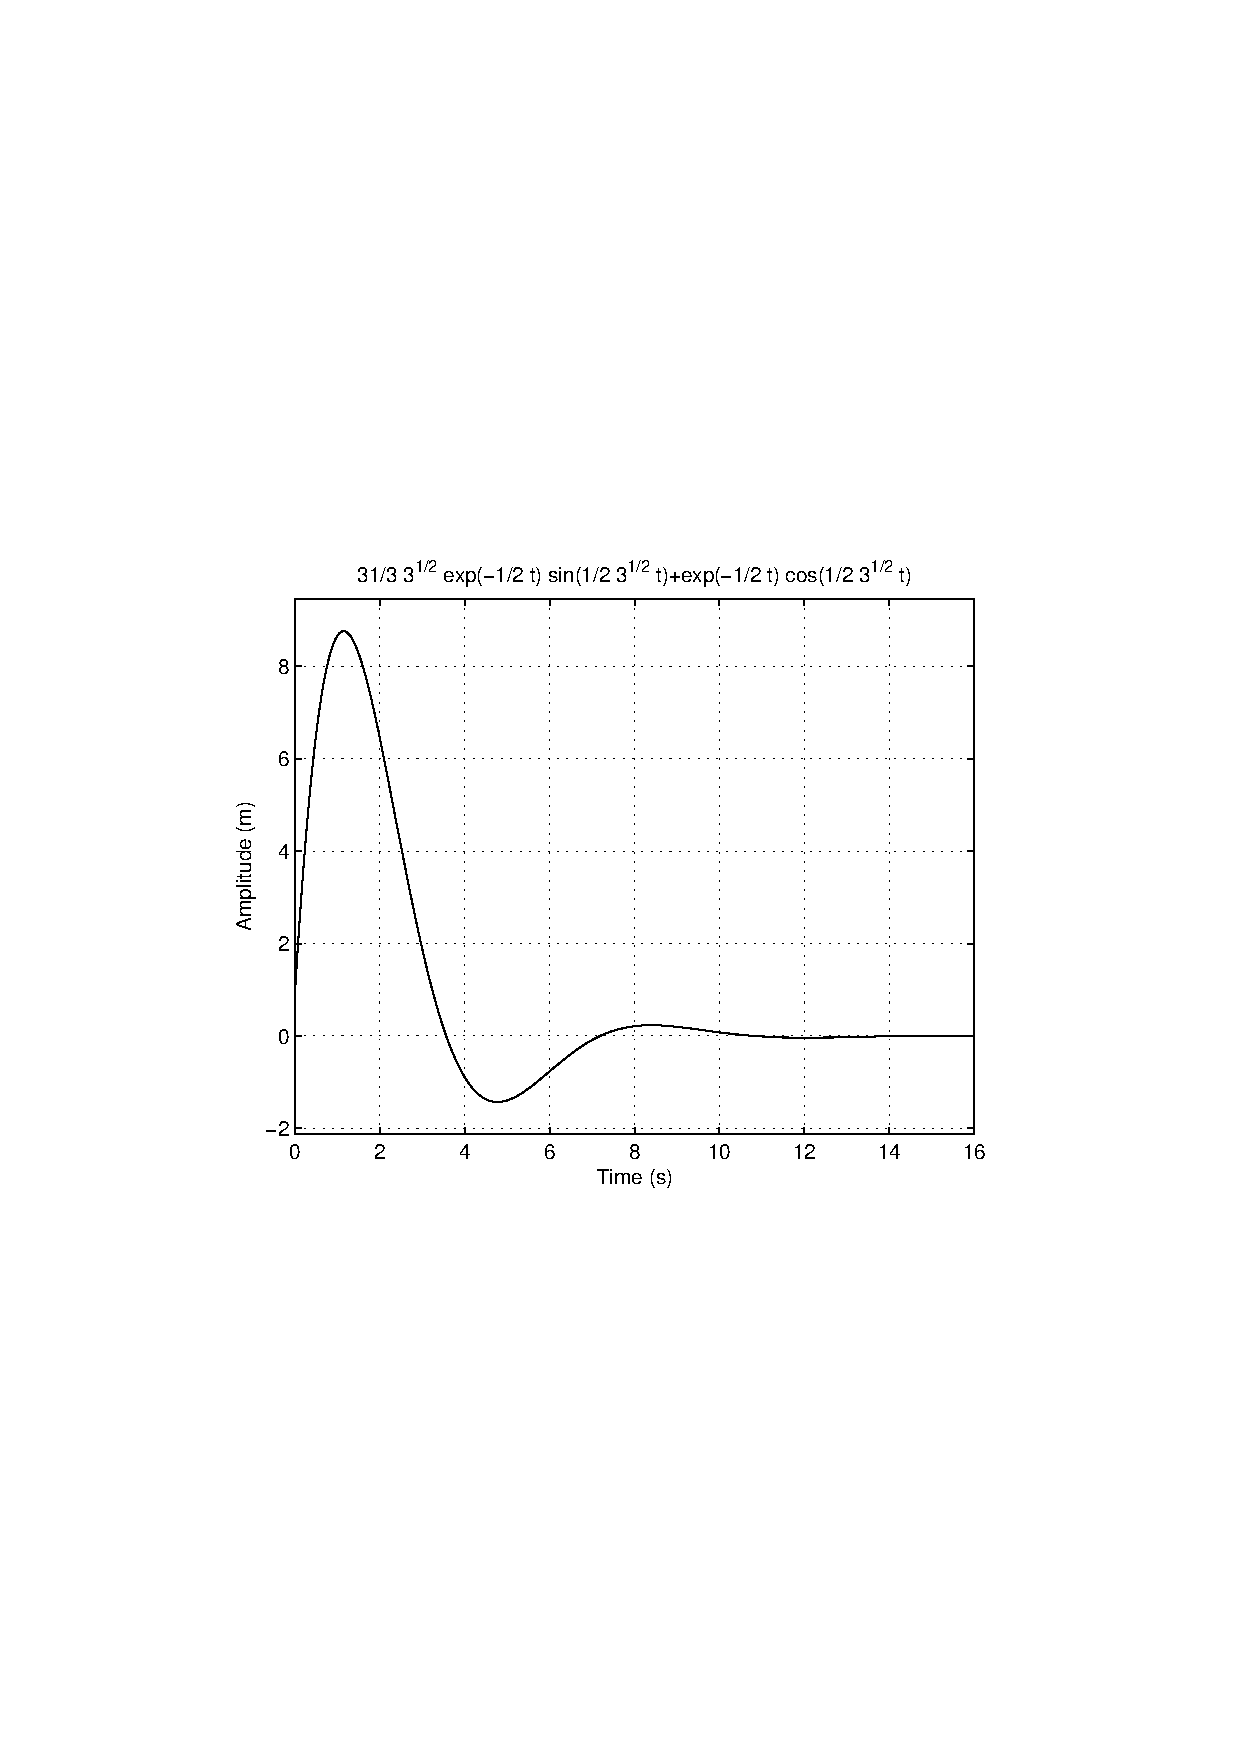
\includegraphics[width=0.7\textwidth]{tlmosc}
\caption{Grafické zobrazenie riešenia rovnice \ref{r:1}}\label{o:2}
\end{figure}



\subsection{Podkapitola}
Podkapitoly záverečnej práce majú za úlohu členenie textu záverečnej
práce s~cieľom, čo najväčšej prehľadnosti. Kapitol môže byť viacero
a~v~ich názvoch sa používa desatinné číslovanie.
%
%!TEX root = tukedip.tex
\section{Jadro pr\'ace}

Začnime rovnicou

\begin{equation}\label{r:2}
\frac{\ud^2y}{\ud t^2}+\frac{\ud y}{\ud t}+y =0, \qquad y(0)=1, \quad
y\,'(0)=15.
\end{equation}

Grafický priebeh riešenia tejto rovnice vidíme na Obrázku \ref{o:2}.

\begin{figure}[ht!]
\centering
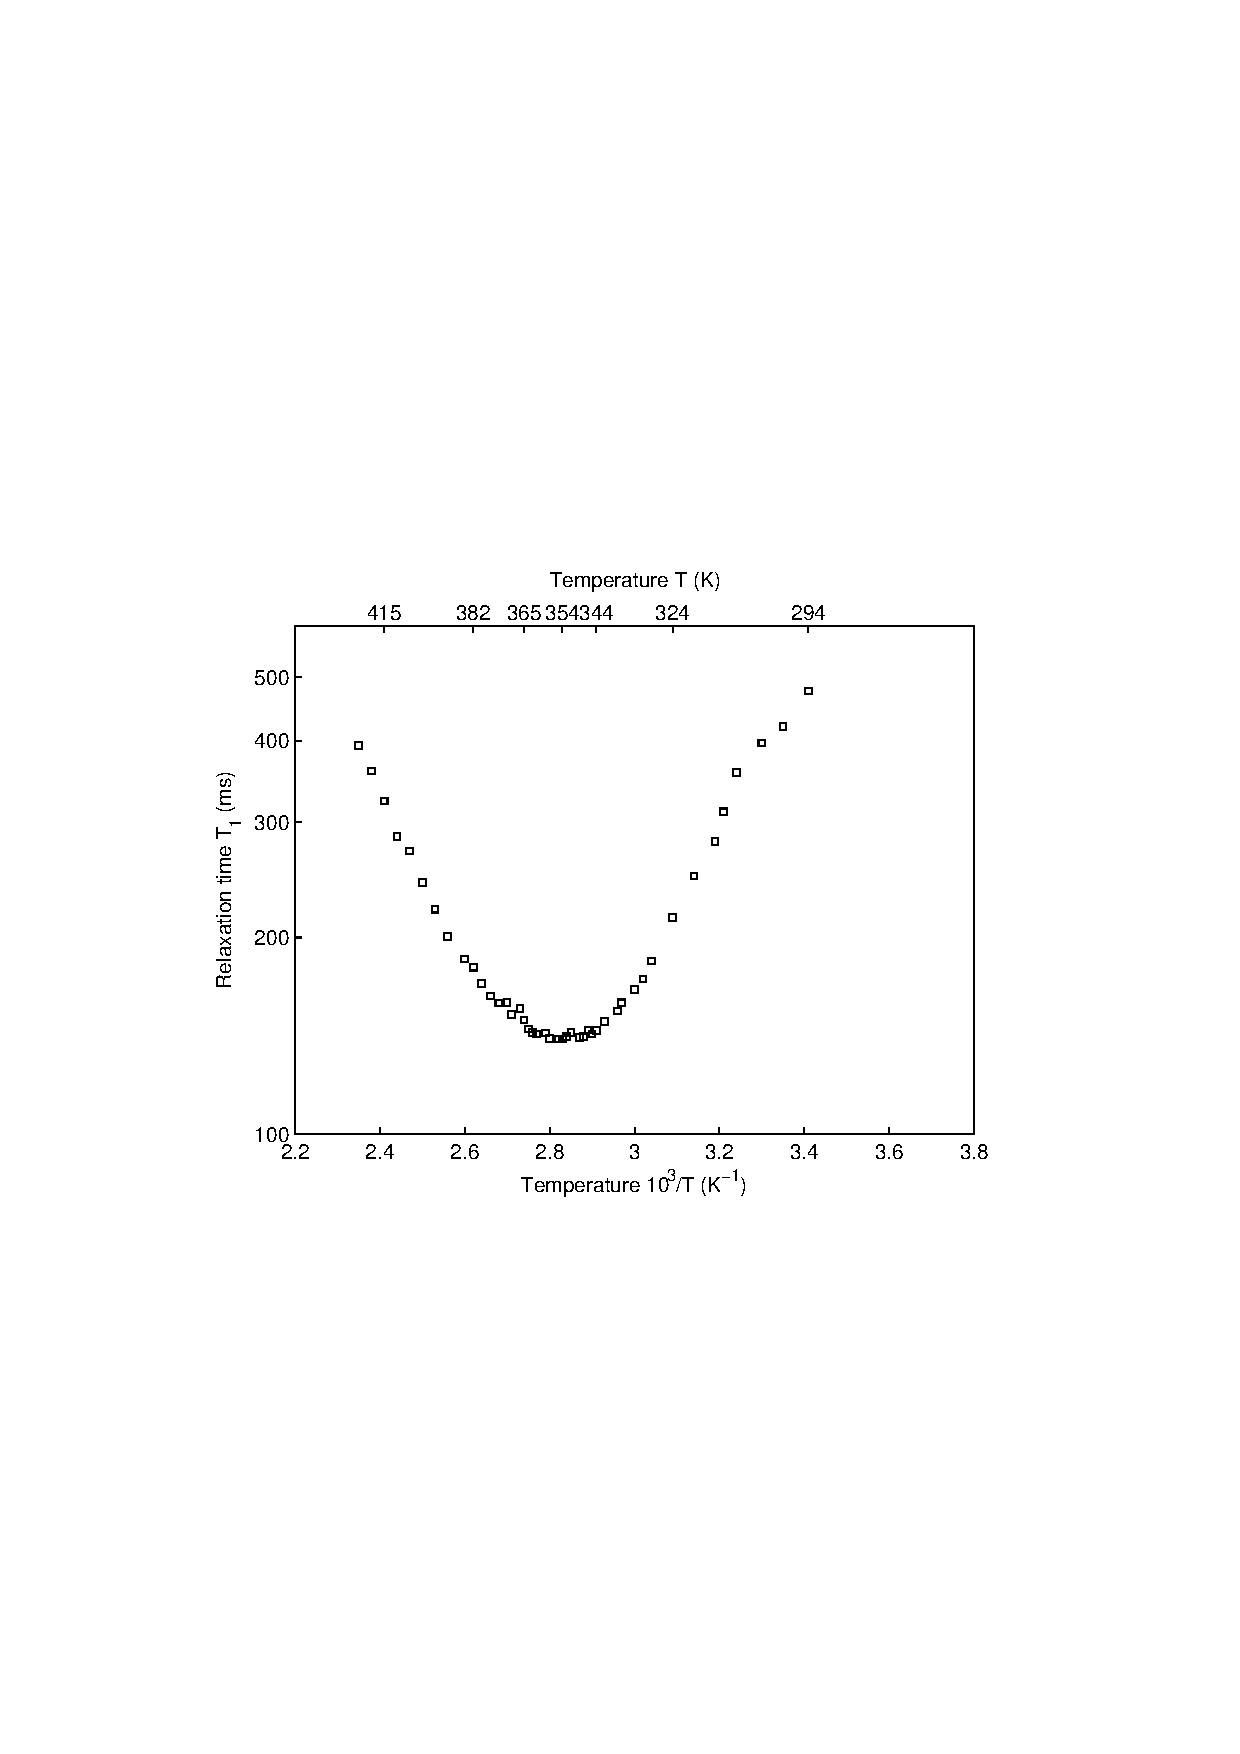
\includegraphics[width=.6\textwidth,angle=0]{relaxcas.pdf}
\caption{Teplotná závislosť\/ spinovo-mriežkového relaxačného
času}\label{o:3}
\end{figure}

%\tabcolsep=3pt % sirka stlpcov
%\renewcommand{\arraystretch}{1.2} % riadkovanie
\begin{table}[ht!]
\centering
\caption{Parametre získané z~meraní spinovo-mriežkových relaxačných
časov $T_1$}\label{t:2}
\medskip
\newcolumntype{d}{D{,}{,}{-1}}
\begin{tabular}{||c||d|d|d|d|d||}
\hhline{|t:==t:==:==:t|}
\multicolumn{1}{||c||}{}&\multicolumn{1}{c|}{PP --
01}&\multicolumn{1}{c|}{PP -- 05}&\multicolumn{1}{c|}{PP --
10}&\multicolumn{1}{c|}{PP -- 16}&\multicolumn{1}{c||}{PP -- 22} \\
\hhline{|:==:==:==:|}
C $\cdot 10^8$~(s$^{-2}$) & 10,1 & 10,0 & 11,0 & 9,2 & 8  \\
\hhline{||-|-|-|-|-|-||}
$\tau_0 \cdot 10^{-14}$~(s) & 2,63 & 1,44 & 0,95 & 2,21 & 10,83  \\
\hhline{||-|-|-|-|-|-||}
$E_{\text a}$~(kJ) & 34,26 & 8,33 & 39,76 & 37,31 & 31,86  \\
\hhline{||-|-|-|-|-|-||}
$T_{\min}$~(K) & 354 & 367 & 367 & 369 & 367  \\
\hhline{||-|-|-|-|-|-||}
$T_{1\min}$~(ms) & 141 & 160 & 157 & 175 & 181  \\
\hhline{||-|-|-|-|-|-||}
$\Delta M_2$~(Gs$^2$) & 5,49 & 5,66 & 5,16 & 5,09 & 5,02  \\
\hhline{|b:==b:==:==:b|}
\end{tabular}
\end{table}


%
%!TEX root = tukedip.tex
\section{Z\'aver (zhodnotenie rie\v{s}enia)}

Tátto časť\/ záverečnej práce je povinná. Autor uvedie zhodnotenie
riešenia. Uvedie výhody, nevýhody riešenia,  použitie výsledkov, ďalšie
možnosti a~pod., prípadne načrtne iný spôsob riešenia úloh, resp.
uvedie, prečo postupoval uvedeným spôsobom.
%
%%
\begin{thebibliography}{999}
\addcontentsline{toc}{section}{\numberline{}Zoznam pou\v{z}itej
literat\'ury}

\harvarditem{Barančok et al.}{1995}{barancok}
BARANČOK, D. et al. 1995. \emph{The effect of semiconductor surface
treatment on LB film/Si interface.} In:~Physica Status Solidi (a), 
ISSN 0031-8965, 1995, vol. 108, no.~2, \mbox{pp. K~87--90}

\harvarditem{Benčo}{2001}{benco}
BENČO, J. 2001. \emph{Metodológia vedeckého výskumu.} Bratislava~:
IRIS, 2001, ISBN 80\discretionary{-}{-}{-}89018-27-0

\harvarditem{Gonda}{2001}{gonda}
GONDA, V. 2001. \emph{Ako napísať a~úspešne obhájiť diplomovú prácu.}
Bratislava~: Elita, 2001, 3. doplnené a~prepracované vydanie, 120~s.
ISBN 80-8044-075-1

\harvarditem{Jadr. fyz. a~tech.}{1985}{slovnik}
\emph{Jadrová fyzika a~technika: Terminologický výkladový slovník.}
2.~rev.~vyd. Bratislava~: ALFA, 1985. 235~s. ISBN 80-8256-030-5

\harvarditem{Katuščák}{1998}{kat}
KATUŠČÁK, D. 1998. \emph{Ako písať vysokoškolské a~kvalifikačné
práce.} Bratislava~: Stimul, 1998, 2.~doplnené vydanie. 121~s. ISBN
80-85697-82-3

\harvarditem{Lamoš a~Potocký}{1989}{lamos}
LAMOŠ, F. -- POTOCKÝ, R. 1989. \emph{Pravdepodobnosť a~matematická
štatistika.} 1.~vyd. Bratislava~: Alfa, 1989. 344~s. ISBN 80-8046-020-5

\harvarditem{Sýkora a~i.}{1980}{sykora}
SÝKORA, F. a~iní. 1980. \emph{Telesná výchova a~šport.} 1.vyd.
Bratislava~: SPN, 1980. 35~s. ISBN 80-8046-020-5

\harvarditem{Steinerová}{2000}{steinerova}
STEINEROVÁ, J. 2000. \emph{Základy filozofie človeka v~knižničnej
a~informačnej vede.} In:~Kimlička, Š., Knižničná a~informačná veda na
prahu informačnej spoločnosti. Bratislava~: Stimul, 2000. ISBN
80-2274-035-2, s. 327--334

\harvarditem{Šumichrast}{1995}{sumichrast}
ŠUMICHRAST, Ľ. 1995. \emph{On the performance of higher approximations
of radiation boundary conditions for the simulation of wave propagation
in structures of integrated optics.} In:~Photonics '95. Prague~: CTU,
1995, pp. 159--161
\end{thebibliography}
%
\section*{Zoznam pr\'iloh}
\addcontentsline{toc}{section}{\numberline{}Zoznam pr\'iloh}
\thispagestyle{empty}

\begin{description}
	\item[Príloha A] Prílohy
	\item[Príloha B] Bibliografické odkazy
	\item[Príloha C] Vytvorenie zoznamu skratiek a symbolov
	\item[Príloha D] 
\end{description}
%
\section*{Pr\'iloha A}
\addcontentsline{toc}{section}{\numberline{}Pr\'iloha A}
\subsection*{Pr\'ilohy}

Táto časť\/ záverečnej práce je povinná a~obsahuje zoznam všetkých
príloh vrátane elektronických nosičov. Názvy príloh v~zozname musia
byť\/ zhodné s~názvami uvedenými na príslušných prílohách. Tlačené
prílohy majú na prvej strane identifikačné údaje -- informácie zhodné
s~titulnou stranou záverečnej práce doplnené o~názov príslušnej
prílohy. Identifikačné údaje sú aj na priložených diskoch alebo
disketách. Ak je médií viac, sú označené aj číselne v~tvare $I/N$, kde
$I$ je poradové číslo a~$N$ je celkový počet daných médií. Zoznam
príloh má nasledujúci tvar:
\begin{description}
\item[Príloha A] CD médium -- záverečná práca v~elektronickej podobe,
prílohy v~elektronickej podobe.
\item[Príloha B] Používateľská príručka
\item[Príloha C] Systémová príručka
\end{description}
Prílohová časť\/ je samostatnou časťou kvalifikačnej práce. Každá
príloha začína na novej strane a je označená samostatným písmenom
(Príloha A, Príloha B, \dots). Číslovanie strán príloh nadväzuje na
číslovanie strán v~hlavnom texte. Pri každej prílohe sa má uviesť\/
prameň, z~ktorého sme príslušný materiál získali.
%
\section*{Pr\'iloha B}
\addcontentsline{toc}{section}{\numberline{}Pr\'iloha B}
\subsection*{Bibliografick\'e odkazy}

Táto časť\/ záverečnej práce je povinná. V~zozname použitej literatúry
sa uvádzajú odkazy podľa normy STN~ISO~690--2 (01 0197) (Informácie
a~dokumentácia. Bibliografické citácie. Časť\/ 2: Elektronické
dokumenty alebo ich časti, dátum vydania 1.~12.~2001, ICS:~01.140.20).
Odkazy sa môžu týkať\/ knižných, časopiseckých a~iných zdrojov
informácií (zborníky z~konferencií, patentové dokumenty, normy,
odporúčania, kvalifikačné práce, osobná korešpondencia a~rukopisy,
odkazy cez sprostredkujúci zdroj, elektronické publikácie), ktoré boli
v~záverečnej práci použité.

Forma citácií sa zabezpečuje niektorou z~metód, opísaných v~norme
STN~ISO~690, 1998, s.~21. Podrobnejšie informácie nájdete na stránke
\texttt{http://www.tuke.sk/anta/} v~záložke {\small\sf Výsledky
práce/Prehľad normy pre publikovanie STN~ISO~690 a~STN~ISO~690-2}.

Existujú dva hlavné spôsoby citovania v~texte.

\begin{itemize}
\item Citovanie podľa mena a~dátumu.
\item Citovanie podľa odkazového čísla.
\end{itemize}

\emph{Preferovanou metódou citovania} v~texte vysokoškolskej
a~kvalifikačnej práce je podľa normy ISO~7144 citovanie podľa mena
a~dátumu \citep{kat,gonda}. V~tomto prípade sa zoznam použitej
literatúry upraví tak, že za meno sa pridá rok vydania. Na uľahčenie
vyhľadávania citácií sa zoznam vytvára v~abecednom poradí autorov.

\medskip

Príklad:
\dots podľa \citep{steinerova} je táto metóda dostatočne rozpracovaná
na to, aby mohla byť\/ všeobecne používaná v~\dots

\medskip

Druhý spôsob uvedenia odkazu na použitú literatúru je uvedenie len
čísla tohto zdroja v~hranatých zátvorkách bez mena autora (autorov)
najčastejšie na konci príslušnej vety alebo odstavca.

\medskip

Príklad:
\dots podľa [13] je táto metóda dostatočne rozpracovaná na to, aby
mohla byť\/ všeobecne používaná v~\dots ako je uvedené v~[14].

\medskip

Citácie sú spojené s~bibliografickým odkazom poradovým číslom v~tvare
indexu alebo čísla v~hranatých zátvorkách. Odkazy v~zozname na konci
práce budú usporiadané podľa týchto poradových čísel. Viacero citácií
toho istého diela bude mať\/ rovnaké číslo. Odporúča sa usporiadať\/
jednotlivé položky v~poradí citovania alebo podľa abecedy.

\medskip
\noindent
Rôzne spôsoby odkazov je možné dosiahnuť\/ zmenou voľby v~balíku
\verb+natbib+:

\noindent
\verb+% Citovanie podla mena autora a roku+\\
\verb+\usepackage[]{natbib}\citestyle{chicago}+\\
\verb+% Možnosť rôznych štýlov citácií. Príklady sú uvedené+\\
\verb+% v preambule súboru natbib.sty.+\\
\verb+% Napr. štýly chicago, egs, pass, anngeo, nlinproc produkujú+\\
\verb+% odkaz v tvare (Jones, 1961; Baker, 1952). V prípade, keď+\\
\verb+% neuvedieme štýl citácie (vynecháme \citestyle{}) v "options"+\\
\verb+% balíka natbib zapíšeme voľbu "colon".+

\medskip
\noindent
Keď zapneme voľbu \verb+numbers+, prepneme sa do režimu citovania
podľa odkazového čísla.

\noindent
\verb+% Metoda ciselnych citacii+\\
\verb+\usepackage[numbers]{natbib}+

\bigskip

Pri zápise odkazov sa používajú nasledujúce pravidlá:

V~odkaze na knižnú publikáciu (pozri príklad zoznamov na konci tejto
časti):
\begin{itemize}
\item Uvádzame jedno, dve alebo tri prvé mená oddelené pomlčkou,
ostatné vynecháme a~namiesto nich napíšeme skratku et al. alebo a~i.
\item Podnázov sa môže zapísať\/ vtedy, ak to uľahčí identifikáciu
dokumentu. Od názvu sa oddeľuje dvojbodkou a~medzerou.
\item Dlhý názov sa môže skrátiť\/ v~prípade, ak sa tým nestratí
podstatná informácia. Nikdy sa neskracuje začiatok názvu. Všetky
vynechávky treba označiť\/ znamienkami vypustenia  \uv{\dots}
\end{itemize}

Pri využívaní informácií z~elektronických dokumentov  treba
dodržiavať\/ tieto zásady:
\begin{itemize}
\item  uprednostňujeme autorizované súbory solídnych služieb
a~systémov,
\item zaznamenáme dostatok informácií o~súbore tak, aby ho bolo opäť\/
možné vyhľadať\/,
\item urobíme si kópiu použitého prameňa v~elektronickej alebo
papierovej forme,
\item za verifikovateľnosť\/ informácií zodpovedá autor, ktorý sa na
ne odvoláva.
\end{itemize}

Pre zápis elektronických dokumentov platia tie isté pravidlá, ako pre
zápis \uv{klasických}. Navyše treba uviesť\/ tieto údaje:
\begin{itemize}
\item  druh nosiča  [online], [CD-ROM], [disketa], [magnetická páska]
\item dátum citovania  (len pre online dokumenty)
\item dostupnosť\/  (len pre online dokumenty)
\end{itemize}

Poradie prvkov odkazu je nasledovné:
Autor. Názov. In Názov primárneho zdroja: Podnázov. [Druh  nosiča].
Editor. Vydanie alebo verzia. Miesto vydania : Vydavateľ, dátum
vydania. [Dátum citovania]. Poznámky.  Dostupnosť\/. ISBN alebo ISSN.
%
\section*{Pr\'iloha C}
\addcontentsline{toc}{section}{\numberline{}Pr\'iloha C}
\subsection*{Vytvorenie zoznamu skratiek a symbolov}

Ak sú v~práci skratky a symboly, vytvára sa \emph{Zoznam skratiek
a~symbolov} (a~ich dešifrovanie). V~prostredí \LaTeX{}u sa takýto
zoznam
ľahko vytvorí pomocou balíka \verb+nomencl+. Postup je nasledovný:
\begin{enumerate}
\item Do preambuly zapíšeme nasledujúce príkazy\\
\verb+\usepackage[slovak,noprefix]{nomencl}+\\ \verb+\makeglossary+
\item  V~mieste, kde má byť\/ vložený zoznam zapíšeme príkaz\\
\verb+\printglossary+
\item V miestach, kde sa vyskytujú skratky a symboly ich definíciu
zavedieme, napr. ako     	v~našom texte, príkazmi\\
\verb+\nomenclature{$\upmu$}{mikro, $10^{-6}$}+\\
\verb+\nomenclature{V}{volt, základná jednotka napätia v sústave SI}+\\
a dokument \uv{pre\LaTeX{}ujeme}.
\item Z~príkazového riadka spustíme program \verb+makeindex+
s~prepínačmi podľa použitého operačného systému, napr.~v~OS~GNU/Linux
s~distribúciou Ubuntu~$10.04$ a~verziou \verb+texlive 2009-7+
napíšeme:\\
\verb*+makeindex tukedip.glo -s nomencl.ist -o tukedip.gls+
\item Po opätovnom \uv{pre\LaTeX{}ovaní} dokumentu sa na
požadované
miesto vloží \emph{Zoznam skratiek a symbolov}.
\end{enumerate}

%
% zivotopis autora
\curriculumvitae\protect\label{page:posledna}
Táto časť\/ je nepovinná. Autor tu môže uviesť\/ svoje biografické
údaje, údaje o~záujmoch, účasti na~projektoch, účasti na~súťažiach,
získané ocenenia, zahraničné pobyty na~praxi, domácu prax, publikácie
a~pod.
\kcurriculumvitae

\end{document}
%%